\chapter{Evaluation}
\label{ch:Evaluation}
In this chapter, we evaluate the contributions of this thesis and the general state of the project. On that account, we first examine the changes to the UI, the Source Code Tooltips, and performance improvements. We then verify the most important features of the CRI by checking a set of specifications for each test application and discussing the result.

All performance measurements and tests in this chapter were performed with Chrome Version 64.0.3282.140 (Official Build) 64-bit, WebStorm 2017 3.4 and Windows 10 Home 64-bit version 1709 build 16299.192. The used device has 8GB RAM, Intel i7 7500 2.7GHz 4CPUs Processor with integrated Intel(R) HD Graphics 620. Each test application was hosted on the integrated Web server of WebStorm on the local machine. No other applications were running during the execution of the tests, although, background processes and services, as well as, other unpredictable factors have to be taken into account which may have influenced the results of the performance measurements.

\section{Evaluation of Improvements}
This section examines the improvements introduced by this thesis and their implementations. We inspect the changes made to the UI as well as the Source Code Tooltips and their applicability regarding the test applications. At last, we examine the performance improvements introduced by this thesis in comparison with the previous version of the CRI.

	\subsection{Changes to the User Interface}
	Most of the changes to the User Interface are, by their nature, hard to evaluate in regards to their usability improvements. The experienced usability of a UI can be highly subjective. The easiest way to achieve consistent evaluation results is, therefore, by collecting and analyzing empirical data, for example through Clickstream analysis \cite{Clickstream}. Since the CRI is not yet used in active production systems by a large user base, a User Study would be the usual approach but would exceed the scope of this thesis. However, some changes are still verifiable as improvements. For example, the text per node in the dependency graph was reduced without losing any information. This is clearly a general improvement of usability because the change did not affect any other part of the UI and removed obsolete text. 
	In addition to highlighting a node that was updated in the currently viewed step of the dependency graph history, edge highlighting now provides additional information for the user. This helps track down differences between steps which were not as easily detectable before without affecting other aspects of the UI. Furthermore, there is now an option - the \emph{hide} button - to hide parts of the UI which are not necessary to examine the dependency graph. Although the \emph{hide} button as a new UI element might introduce minor usability issues, it can still be considered an objective improvement - as can the edge highlighting.
	
	%TODO continue

	\subsection{Inspecting Source Code Tooltips}
	The Source Code Tooltips that connect nodes in the dependency graph with the JS code they originate from are created whenever the user hovers over a node and presses the CTRL key. Due to their on-demand nature, their performance impact on the time-critical computations of the CRI like the recording process can be neglected. The original JS files are stored in a variable in a content script of the CRI that is queried for the lines corresponding to a node if requested. Storing a copy of the whole JS file in addition to the instrumented version, however, should not exceed the memory (i.e. Random Access Memory) of any modern computer that runs Google Chrome. We will examine the robustness of this feature in regards to its accuracy in a later section as part of the test application evaluation. To investigate and verify the usefulness of Source Code Tooltips we examined each test application and calculated the percentage of nodes that gain additional context through this feature. As a \emph{named} node already has some form of context that helps the user to identify it and its dependents, we counted \emph{named} nodes separately. For the exact circumstances and inputs used for each test application see section \ref{sec:EvalTests}. %TODO rephrase Over all? remove paragraph
	 Over all test applications, there were 586 nodes in total. Of these, 440 nodes had a Source Code Tooltip which equals to approximately 75\% of all nodes. Only 199, approximately 33.9\% of all nodes are \emph{named}. This means that the introduction of Source Code Tooltips provided additional means to identify a node to the user for 35.1\% of the total number of nodes. The remaining 146 nodes that cannot yet be linked to specific positions in the source code in part consist of nodes that can be easily interpreted by examining the nodes that depend on them. For example in the test application \emph{RXJS canvas-painting} the node with Id 6 is a \emph{FromEventObservable} created by "Rx.Observable.fromEvent(colorchar,"click")" and is not yet detected by the Jalangi analysis.

	\subsection{Scrutinizing Performance with rapidly updated Observables}
	\label{sec:PerformanceEvaluation}
	In this section, we evaluate the performance improvements resulting from the reworked graph history and the less frequent UI rendering in detail. To this purpose, we developed a new test application for RxJS which is used as a simple benchmark on how well the CRI, and in the last part of this section RxFiddle, cope with a simple rapidly updating observable. The application uses an \emph{interval observable} to generate one update every five milliseconds over a period of five seconds. Listing \ref{lst:performanceTestExtract} shows the observable responsible for the updates. The full source code including the termination after five seconds is presented in Appendix \ref{ch:Appendix}.
	
	\begin{lstlisting}[language=JavaScript, caption={Example of RxJS code.},label={lst:performanceTestExtract}]
	var intervalObservable = Rx.Observable.interval(5)
	.timestamp()
	.bufferCount(2, 1)
	.map(function (w) {
	return w[1].timestamp - w[0].timestamp;
	})
	.share();	
	\end{lstlisting}

	To exclude the initial setup of the CRI from the gathered performance data we create a \emph{reactive breakpoint} for the \emph{nodeCreated} event of node one ("nodeCreated[1]"), ran the application until it paused at the \emph{reactive breakpoint}, started the performance recording and then continued execution. To record a CPU profile that includes the time spent per function we used the Chrome-JavaScript Profiler. To inspect the memory usage we used the memory tab of Chrome DevTools. The duration of the recordings vary from the actual execution time of the test application in the respective case, because they were started and ended manually. 
	
	\textbf{CPU Profile}
	\begin{figure}[!h]
	\centering
	\subfloat[Chrome Reactive Inspector version 2.0]{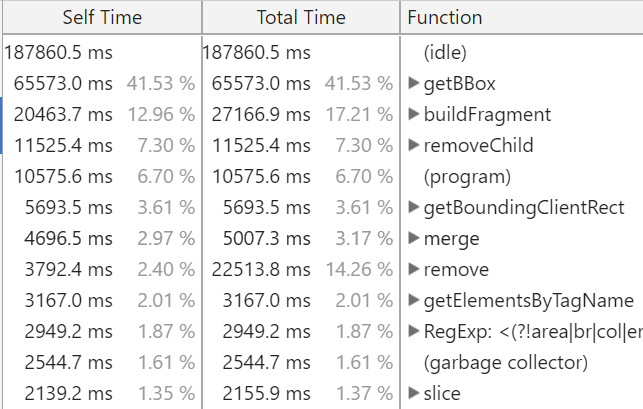
\includegraphics[width=0.49\textwidth]{gfx/CPU_CRI2.png}\label{fig:CPUCRI2}}
	\hfill
	\subfloat[Chrome Reactive Inspector version 3.0]{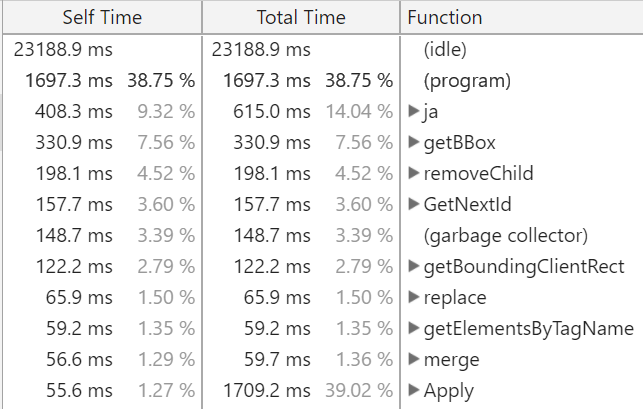
\includegraphics[width=0.49\textwidth]{gfx/CPU_CRI3.png}\label{fig:CPUCRI3}}
	\caption{CPU Profiles recorded by Google Chrome's JavaScript Profiler.}
	\end{figure}
	
	The label "(program)" in the recording entitles native code execution of Chrome. The measured execution time for this label is far less accurate than any other measurement because the individual composition is unclear and can solely increase by stopping the recording at a later point in time due to the limitations of the recording tool.
	
	For the CRI2 the execution of \emph{PerformanceTest} took approximately 154.0 seconds with an overall recording interval of 187.9 seconds. To differentiate between execution time and recording time we selected an area with significantly higher CPU load that should correspond reasonably well to the actual execution time. The largest percentage of \emph{self time}, i.e. the time spent executing code directly in a function itself, that was spent in a single function directly corresponds to excessive UI updates. These updates happen at least once per created step in the history since the slider is updated and triggers the rendering of a new dependency graph for that step. \emph{getBB} (getBoundingBox) calculates the size of nodes in the graph, whereas  \emph{buildFragment}'s impact stems from the \emph{domManip} function of jQuery.\\
	For the CRI3 the execution took approximately 5.5 seconds with an overall recording interval of 23.2 seconds. It is visible that still a sizable amount of time is spent inside UI related computations especially \emph{getBB}. The most time of execution not related to Chromes native code is spent inside the \emph{ja} function of jQuery that cannot easily be tracked down to corresponding CRI code. Overall the most time is spent inside Chromes native code, but as described earlier this can have numerous reasons. Due to the nature of changes from the CRI2 to the CRI3 we are, however, able to account at least part of that execution time to storage operations using the Chrome Storage API. 
	As the CRI3 was approximately 28 times faster than the CRI2, the performance improvements regarding rapidly updated observables implemented by this thesis were effective. It is, however, worth noting, that the CRI2 is barely able to handle this test without crashing - the UI becomes temporarily unresponsive. This probably increases the performance differences between the two versions of the CRI more than they are for a test both CRI versions handle well, i.e. without the UI becoming temporarily unresponsive. We chose to keep the test as-is to underline the impact of \emph{request buildup} and of load exceeding the extension's capacity.
	As of now the CRI3 also has a fixed capacity of updates it is able to handle without crashing, but it is much higher than the CRI2's mostly due to the throttling of rendering operations. In the future the CRI should be extended to automatically detect if rendering computations accumulate beyond its limit and increase or decrease the throttle interval for UI updates accordingly. Since all steps are recorded even if the rendering is not able to keep up, increasing the throttle time to keep the extension from crashing is a viable approach. The user is then able to pause the recording anytime and examine the steps in details whereas a crash will render the CRI useless to the user.
	
	\textbf{Memory Profiling}\\
	To reveal the impact of a large history on the memory consumption of the CRI we executed \emph{PerformanceTest} with a limit of 250ms for both versions of the CRI in addition to the execution we used for CPU profiling with a limit of five seconds.
	\begin{figure}[!h]
		\centering
		\subfloat[CRI2 - 5s duration]{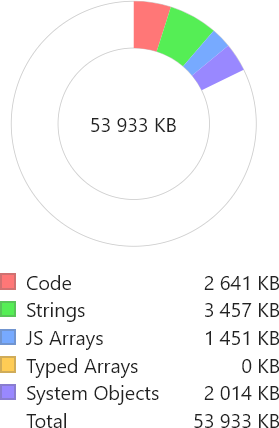
\includegraphics[width=0.3\textwidth]{gfx/RAM_CRI2.png}\label{fig:RAM2}}
		\hspace{1cm}
		\subfloat[CRI3 - 5s duration]{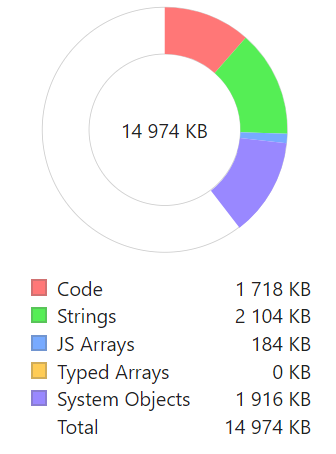
\includegraphics[width=0.3\textwidth]{gfx/RAM_CRI3.png}\label{fig:RAM3}}
		\hspace{10cm} % forces the linebreak between images
		\subfloat[CRI2 - 250ms duration]{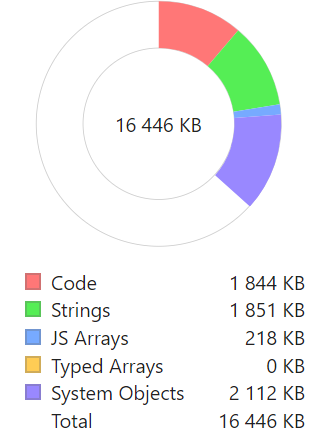
\includegraphics[width=0.3\textwidth]{gfx/RAM_CRI2_250ms.png}\label{fig:RAM2Short}}
		\hspace{1cm}
		\subfloat[CRI3 - 250ms duration]{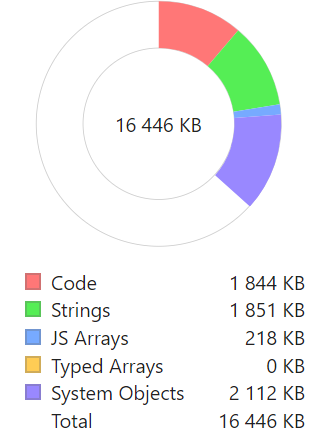
\includegraphics[width=0.3\textwidth]{gfx/RAM_CRI2_250ms.png}\label{fig:RAM3Short}}
		\caption{Memory Profiles of the CRI during the execution of \emph{PerformanceTest} recorded and displayed by Google Chrome's Memory DevTool.}
	\end{figure}
	For the test execution with the full duration (results visible in figures \ref{fig:RAM2} and \ref{fig:RAM3}) the CRI2 used 52.7MB in total while the CRI3 used only 14.6MB. The most notable difference in a specific category is the size of the memory used by JS arrays which include the stored dependency graph. In the test with reduced execution time (250ms), the CRI2 used approximately 16.1MB of memory while the CRI3 used 12.6MB of memory. Both versions of the CRI have a similar memory consumption for the test with reduced execution time, although the CRI2 shows the dependency graph with a noticeable delay (still less than 5s). Since the CRI3's history implements a stream like approach through paging, the memory usage once the size of a single \emph{page} is exceeded is fairly constant and does not increase with the number of steps. As the CRI2's history does not support paging the memory usage increases approximately proportional to the number of steps in the history. However, since modern computers have usually more than 1GB of memory, even the higher memory consumption of the CRI2 does not have any influence on the overall performance detectable by the user. We made no distinction of the CRI3 with Delta Encoding and Paging; and the CRI3 just with Paging, because this examination shows that the memory usage is far to low to imposes any limitation on the overall performance of the CRI, even for the CRI2. As there were no significant changes to the recording process of RxJS and BaconJS in the CRI, we did not execute separate performance measurements for a test application using BaconJS.
	
	\textbf{Comparison to RxFiddle}\\
	We also examined the performance of RxFiddle with the used test application and compared it to the CRI3 to qualify the discussion in section \ref{sec:RxFiddle} on its performance with rapidly updated observables.
	Although RxFiddle does not have performance issues  with \emph{PerformanceTest} executed in Google Chrome, i.e. not exceeding a delay of one second when hovering over a node before the tooltip is shown, if executed with Firefox (57.0.4 (64-bit)) the browser becomes unresponsive for a few seconds. The overall memory consumption of RxFiddle during the test was 52.5MB and the execution took approximately 5.5 seconds - similar to the CRI3. As mentioned earlier, this magnitude of memory consumption is not a limiting factor for the overall performance. The CRI generates approximately 2700 steps during the test execution while RxFiddle generates approximately one thousand values for each operator in the chain of \emph{intervalObservable} which is displayed in figure \ref{fig:RxFiddlePerformance}. Examining these results any further does not provide additional insight since the tools are based on completely different technologies. RxFiddle uses TypeScript and runs as a Web page while the CRI does not use TypeScript, any form of bundling, or minifying and runs as a Chrome extension.
	\begin{figure}[!h]
		\centering
		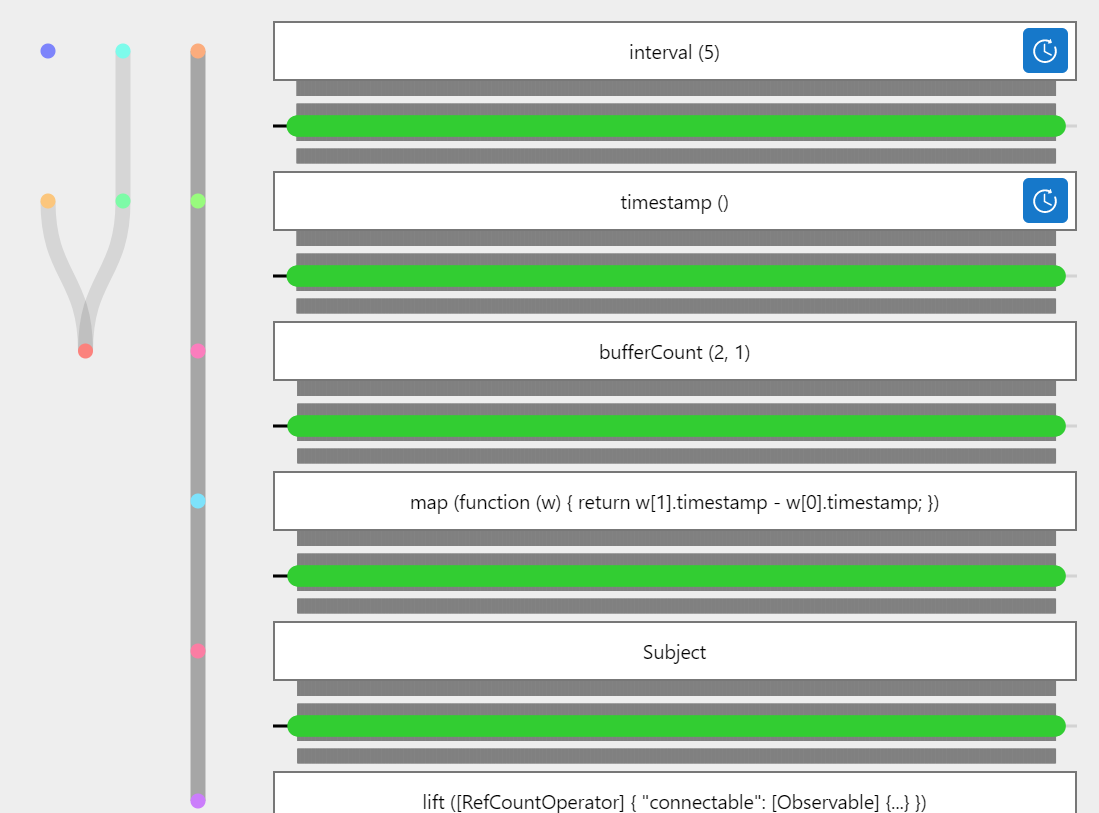
\includegraphics[scale=0.7,trim=0 0 0 0]{gfx/RxFiddleWithTimer.png}
		\caption{Test application PerformanceTest inspected with RxFiddle}
		\label{fig:RxFiddlePerformance}
	\end{figure}
	
\section{Reviewing the Test Applications}
\label{sec:EvalTests}
To establish the current state of the most important features of the CRI we compiled a set of specifications which we validated for each of the test applications. They were designed to provide a baseline for the robustness of the current CRI implementation. Note that we also included specifications targeting features not introduced by this thesis as a means of manual regression testing for the most important aspects of the CRI. Since most of these specifications cannot be tested for each node, step and/or, case in reasonable time, we specified the exact tests we used to approximate the results. These test probes should provide a reasonably precise evaluation which is easy to reproduce in order to verify our results.

\textbf{Specifications}
\begin{itemize}
	\item[Spec1] The dependency graph is shown and all observables that are assigned to a named variable are displayed distinctively. (Test: Up to the first five named observables in the code are all displayed with an orange background.)
	\item[Spec2] The history of the dependency graph can be navigated. It is possible to navigate to the previous, succeeding or a random step in the history. (Test: Jump to the median step; click next five times; click previous five times.)
	\item[Spec3] For each node, no space is occupied by fields that hold no value in neither the node itself nor its tooltip.
	\item[Spec4] The ids of the nodes start at one and are continuous. If the test application is started again with the exact same inputs, each node has the same id as in the last execution.
	\item[Spec5] The Source Code Tooltips show and highlight the corresponding lines of code for each node that has one. (Test: If possible, choose two nodes, one that corresponds to the middle of a chain of reactive function calls and one that corresponds to the end of a chain of reactive function calls. For both nodes check if the highlighting is correct.)
	\item[Spec6] The node or edge that was updated in a step is highlighted. (Test: Check this behavior for the first ten steps in the history.)
	\item[Spec7] The history queries can be used to search for a specific event in the history. (Test: Queries for \emph{evaluationYielded} and \emph{nodeUpdated} find the corresponding steps for the first named node.)
	\item[Spec8] The graph can be searched, the matching node(s) is/are highlighted and if the search is reset the original coloring is restored. (Test: Search for the dependencies and dependents of the first named node and then reset the search.)
	\item[Spec9] \emph{Reactive breakpoints} can be used to pause the debugger when a specific event occurs. (Test: \emph{a)} A breakpoint set for the first node created will break at step one. \emph{b)} A breakpoint for the first node updated will break before the value is updated in the original observable. Note: The value will be already updated in the CRI UI.)
\end{itemize}

We excluded some of the test applications that were used in the prior works targeting the CRI from this evaluation because they no longer function properly due to outside influences or did not provide any additional value. The results of this evaluation are visible in tables \ref{tab:RxJS} and \ref{tab:BaconJS}. For the following statistics, we interpreted \emph{ambiguity} between nodes with the same name, labeled with \emph{Am}, as if the check failed because the CRI is not able to handle them properly yet. \emph{N.A.} specifies that the check was not applicable, for example because there were no \emph{named} nodes in the dependency graph and the check is dependent on \emph{named} nodes. We, therefore, treated \emph{N.A.} as a success. Due to specification number 9 having two parts that can fail or succeed individually we treated their results separately in the following statistic. Overall 388 of 420 single checks (10 per test application) were successful. The specifications number 2 up to number 6 in addition to number 9 \emph{b)} verified for all test applications. The 32 checks that failed have four distinct characteristics. All checks labeled with \emph{ambiguity} are the result of the CRI not being able to handle multiple nodes with the same name. This happens for example if a named variable is created within a loop. The history query and search feature will not be able to correctly distinguish between the ambiguous nodes and any operation that requires a name will only find the node added last to the dependency graph and show the result solely for that node. Specification 9 \emph{a)} failed for all RxJS applications where the node with Id 1 is recorded by the RxJS interception and not by the Jalangi analysis beforehand. It seems the RxJS interception records nodes out of order in certain circumstances. We verified that this behavior already existed in the previous versions of the CRI2 by executing the same check with the \emph{RxJS son-father-wallet} test application with the CRI2. The failed checks for specification number 8 denote fails to identify every dependent or dependency. This seems to correspond to observables being dynamically created but the check will not fail for every dynamically created observable. In case of the check for the \emph{RxJS crop} application, this behavior is not consistent with previous versions of the CRI and stems from changes introduced in the CRI3, however, the issue in the \emph{RxJS stopwatch} application was already present in the CRI2.
In the new test application \emph{RxJS InlineScriptTest}, which was added to verify that the CRI is working with JS code directly embedded within HTML, the CRI does not detect every \emph{named} observable. The reason is that the extension is currently not able to detect and intercept JS code inside HTML attributes.
The failed check for specification number 1 in the \emph{BaconJS blog\_url} test application is the result of BaconJS interception not being able to detect the used observables correctly. The \emph{named} observable is not detected and in addition, each change to the used observable in the JS code creates a new node in the dependency graph. This has to be counted as a complete breakdown of the recording for this test application and is consistent with previous versions of the CRI. The remaining failed check for specification number 1 in the \emph{RxJS alphabetinvasion} application also denotes a full breakdown of the recording. It seems the current implementation is not able to detect the observables correctly or, in most cases, at all. This behavior is also consistent with previous versions of the CRI and is the result of the programming patterns used in this application. The observables which were not recorded correctly are never assigned and no reactive operator or function is used on them except for \emph{subscribe} or \emph{unsubscribe}. Example code that show the described pattern is visible in listing \ref{lst:AlphabetInvasionExtract}. The observable created from the call to "Rx.Observable.timer(750)" is never recorded.

\begin{lstlisting}[language=JavaScript, caption={Extract of RxJS AlphabetInvasion test application.},label={lst:AlphabetInvasionExtract}]
Rx.Observable.timer(750).subscribe(function () {
self.playfield.removeChild(enemy);
});	
\end{lstlisting}

For the test application \emph{RxJS mario} we added a \emph{reactive breakpoint} on the last dependency that is created because the excessive use of timers and rapidly updated observables still causes the CRI to crash after a few seconds. This is probably the result of \emph{request buildup} due to a large number of calls to the communication API of Chrome, but it is hard to provide a sufficient proof because Chrome itself will stop responding as well.

\begin{table}[]
	\centering
	\resizebox{\textwidth}{!}{%
		\begin{tabular}{llllllllll}
			Application              & Spec 1 & Spec 2 & Spec 3 & Spec 4 & Spec 5            & Spec 6 & Spec 7      & Spec 8 & Spec 9                              \\
			alphabetinvasion         & \mno   & \myes  & \myes  & \myes  & \myes             & \myes  & N.A.        & N.A.   & \mno\footnote[3],\myes              \\
			mario                    & \myes  & \myes  & \myes  & \myes  & \myes             & \myes  & \myes       & \myes  & \mno\footnote[3],\myes              \\
			PerformanceTest          & \myes  & \myes  & \myes  & \myes  & \myes             & \myes  & \myes       & \myes  & \mno\footnote[3],\myes              \\
			animated-image           & \myes  & \myes  & \myes  & \myes  & \myes             & \myes  & \myes       & \myes  & \mno\footnote[3],\myes              \\
			animationtest            & \myes  & \myes  & \myes  & \myes  & \myes             & \myes  & \myes       & \myes  & \mno\footnote[3],\myes              \\
			backpressure             & \myes  & \myes  & \myes  & \myes  & \myes             & \myes  & \myes       & \myes  & \mno\footnote[3],\myes              \\
			crop                     & \myes  & \myes  & \myes  & \myes  & \myes             & \myes  & \myes       & \mno   & \mno\footnote[3],\myes              \\
			creaditcard-drag         & \myes  & \myes  & \myes  & \myes  & \myes             & \myes  & \myes       & \mno   & \myes                               \\
			draw-with-combine-latest & \myes  & \myes  & \myes  & \myes  & \myes             & \myes  & \myes       & \myes  & \mno\footnote[3],\myes \footnote[1]{} \\
			earthquake               & \myes  & \myes  & \myes  & \myes  & \myes             & \myes  & N.A., \myes & \myes  & \mno\footnote[3],\myes\footnote[1]{}  \\
			simple-databinding       & \myes  & \myes  & \myes  & \myes  & \myes\footnote[2] & \myes  & \myes       & \myes  & \myes                               \\
			stopwatch                & \myes  & \myes  & \myes  & \myes  & \myes             & \myes  & \myes       & \mno   & \myes                               \\
			subjects-examples        & \myes  & \myes  & \myes  & \myes  & \myes\footnote[2] & \myes  & \myes       & \myes  & \myes                               \\
			wiki-updates             & \myes  & \myes  & \myes  & \myes  & \myes             & \myes  & \myes       & \myes  & \myes                               \\
			smart-counter            & \myes  & \myes  & \myes  & \myes  & \myes             & \myes  & \myes       & \mno   & \mno\footnote[3],\myes              \\
			state-store              & \myes  & \myes  & \myes  & \myes  & \myes             & \myes  & \myes       & \myes  & \mno\footnote[3],\myes              \\
			letter-counter           & \myes  & \myes  & \myes  & \myes  & \myes             & \myes  & \myes       & \myes  & \mno\footnote[3],\myes              \\
			son-father-wallet        & \myes  & \myes  & \myes  & \myes  & \myes             & \myes  & \myes       & \myes  & \mno\footnote[3],\myes              \\
			movie-search             & \myes  & \myes  & \myes  & \myes  & \myes             & \myes  & \myes       & \myes  & \myes                               \\
			follow-the-mouse         & \myes  & \myes  & \myes  & \myes  & \myes             & \myes  & \myes       & \myes  & \myes                               \\
			drag-and-drop            & \myes  & \myes  & \myes  & \myes  & \myes             & \myes  & \myes       & \mno   & \myes                               \\
			canvas-painting          & \myes  & \myes  & \myes  & \myes  & \myes             & \myes  & \myes       & \myes  & \mno\footnote[3],\myes              \\
			twitter-follow-box       & \myes  & \myes  & \myes  & \myes  & \myes             & \myes  & \myes       & \myes  & \myes                               \\
			rest-api-call            & \myes  & \myes  & \myes  & \myes  & \myes             & \myes  & \myes       & \myes  & \mno\footnote[3],\myes              \\
			image-sampler            & \myes  & \myes  & \myes  & \myes  & \myes             & \myes  & \myes       & \myes  & \mno\footnote[3],\myes              \\
			InlineScriptTest         & \mno   & \myes  & \myes  & \myes  & \myes             & \myes  & \myes       & \mno   & \mno\footnote[3],\myes             
		\end{tabular}%
	}
	\caption{Result of checking the specifications for the RxJS test applications}
	\label{tab:RxJS}
\end{table}

\begin{table}[]
	\centering
	\resizebox{\textwidth}{!}{%
		\begin{tabular}{llllllllll}
			Application                       & Spec 1 & Spec 2 & Spec 3 & Spec 4 & Spec 5             & Spec 6 & Spec 7     & Spec 8 & Spec 9 \\
			timer                             & \myes  & \myes  & \myes  & \myes  & \myes              & \myes  & \myes      & \myes  & \myes  \\
			blog\_url                          & \mno   & \myes  & \myes  & \myes  & \myes              & \myes  & N.A.       & N.A.   & \myes  \\
			comb-lock                         & \myes  & \myes  & \myes  & \myes  & \myes              & \myes  & Am         & Am     & \myes  \\
			dragdrop                          & \myes  & \myes  & \myes  & \myes  & \myes              & \myes  & N.A.,\myes & \myes  & \myes  \\
			events                            & N.A.   & \myes  & \myes  & \myes  & \myes \footnote[2] & \myes  & N.A.       & N.A.   & \myes  \\
			operators                         & \myes  & \myes  & \myes  & \myes  & \myes              & \myes  & \myes      & \mno   & \myes  \\
			son-father-wallet split file test & \myes  & \myes  & \myes  & \myes  & \myes              & \myes  & Am         & Am     & \myes  \\
			operators-and-events              & \myes  & \myes  & \myes  & \myes  & \myes              & \myes  & \myes      & \myes  & \myes  \\
			son-father-wallet                 & \myes  & \myes  & \myes  & \myes  & \myes              & \myes  & \myes      & \myes  & \myes  \\
			up-down-counter                   & \myes  & \myes  & \myes  & \myes  & \myes              & \myes  & \myes      & \myes  & \myes  \\
			form-validation                   & \myes  & \myes  & \myes  & \myes  & \myes              & \myes  & \myes      & \myes  & \myes  \\
			movie-search                      & \myes  & \myes  & \myes  & \myes  & \myes              & \myes  & \myes      & \mno   & \myes  \\
			bar-chart                         & \myes  & \myes  & \myes  & \myes  & \myes              & \myes  & \myes      & \myes  & \myes  \\
			websocket-wikipedia               & \myes  & \myes  & \myes  & \myes  & \myes              & \myes  & \myes      & \myes  & \myes  \\
			multiselect-card                  & \myes  & \myes  & \myes  & \myes  & \myes              & \myes  & \myes      & \myes  & \myes  \\
			true-false-logger                 & \myes  & \myes  & \myes  & \myes  & \myes              & \myes  & \myes      & \myes  & \myes  \\
			drawing                           & \myes  & \myes  & \myes  & \myes  & \myes              & \myes  & \myes      & \myes  & \myes 
		\end{tabular}%
	}
	\caption{Result of checking the specifications for the BaconJS test applications}
	\label{tab:BaconJS}
\end{table}
%TODO check table captions
\footnotetext[1]{The node with Id 2 was used because the node with Id 1 is never updated}
\footnotetext[2]{The middle of a reactive function chain could not be examined because no function chain was long enough.}
\footnotetext[3]{The breakpoint pauses program execution at the right step, but since nodes are added out of order the node with Id 2 is already added to the dependency graph}

\subsection{Summary}
We examined the set of specifications for each of the test applications and found several issues. The problems with ambiguous variable names and out-of-order recording of nodes, issues that should be resolved at some point, do not break the overall usefulness of the CRI. This is because the dependency graph can still be examined and other features work as well. In contrast, the issues with recording in the test applications \emph{RxJS alphabetinvasion} and \emph{BaconJS blog\_url} cause the CRI to display an incomplete dependency graph. This greatly reduces the usefulness of the extension with these applications.
All issues found should be the target of further development to increase the robustness of the CRI, but issues in recording observables should clearly be prioritized.